\documentclass[14pt,aspectratio=169]{beamer}
%%%%%%%%%%%%%%%%%%%%%%%%%%%%%%%%%%%%%%%%%%%%%%%%%%%%%%%%%%%%%
% Meta informations:
\newcommand{\trauthor}{Imran Ibrahimli}
\newcommand{\trcourse}{Intelligent Adaptive Systems}
\newcommand{\trtitle}{Length Generalization on Multi-Digit Integer Addition with Transformers}
\newcommand{\trmatrikelnummer}{7486484}
\newcommand{\tremail}{imran.ibrahimli@studium.uni-hamburg.de}
\newcommand{\trinstitute}{Knowledge Technology, WTM \\ Dept. Informatik \\ Universit\"at Hamburg}
\newcommand{\trwebsiteordate}{{19.11.2024}}

%%%%%%%%%%%%%%%%%%%%%%%%%%%%%%%%%%%%%%%%%%%%%%%%%%%%%%%%%%%%%
% Languages:
\usepackage[english]{babel}
\selectlanguage{english}

%%%%%%%%%%%%%%%%%%%%%%%%%%%%%%%%%%%%%%%%%%%%%%%%%%%%%%%%%%%%%
% Bind packages:
\usepackage{beamerthemesplit}
\usetheme{Boadilla}
%\usetheme{Copenhagen}
%\usetheme{Darmstadt}
%\usetheme{Frankfurt}
%\usetheme{Ilmenau}
%\usetheme{JuanLesPins}
%\usetheme{Madrid}
%\usetheme{Warsaw }
%\usecolortheme{dolphin}
%\setbeamertemplate{sections/subsections in toc}[sections numbered]
%\beamertemplatenavigationsymbolsempty
%\setbeamertemplate{headline}[default] 	% deaktiviert die Kopfzeile
\setbeamertemplate{navigation symbols}{}% deaktiviert Navigationssymbole
%\useinnertheme{rounded}

\usepackage{acronym}                    % Acronyms
\usepackage{algorithmic}								% Algorithms and Pseudocode
\usepackage{algorithm}									% Algorithms and Pseudocode
\usepackage{amsfonts}                   % AMS Math Packet (Fonts)
\usepackage{amsmath}                    % AMS Math Packet
\usepackage{amssymb}                    % Additional mathematical symbols
\usepackage{amsthm}
\usepackage{color}                      % Enables defining of colors via \definecolor
\usepackage{fancybox}                   % Gleichungen einrahmen
\usepackage{fancyhdr}										% Paket zur schickeren der Gestaltung der 
\usepackage{graphicx}                   % Inclusion of graphics
%\usepackage{latexsym}                  % Special symbols
\usepackage{longtable}									% Allow tables over several parges
\usepackage{listings}                   % Nicer source code listings
\usepackage{lmodern}
\usepackage{multicol}										% Content of a table over several columns
\usepackage{multirow}										% Content of a table over several rows
\usepackage{rotating}										% Alows to rotate text and objects
\usepackage[section]{placeins}          % Ermoeglich \Floatbarrier fuer Gleitobj. 
\usepackage[hang]{subfigure}            % Allows to use multiple (partial) figures in a fig
%\usepackage[font=footnotesize,labelfont=rm]{subfig}	% Pictures in a floating environment
\usepackage{tabularx}										% Tables with fixed width but variable rows
\usepackage{booktabs}
\usepackage{url,xspace,boxedminipage}   % Accurate display of URLs


\definecolor{uhhRed}{RGB}{226,0,26}     % Official Uni Hamburg Red
\definecolor{uhhGrey}{RGB}{136,136,136} % Official Uni Hamburg Grey
\definecolor{uhhLightGrey}{RGB}{220, 220, 220}
\setbeamertemplate{itemize items}[ball]
\setbeamercolor{title}{fg=uhhRed,bg=white}
\setbeamercolor{title in head/foot}{bg=uhhRed}
\setbeamercolor{block title}{bg=uhhGrey,fg=white}
\setbeamercolor{block body}{bg=uhhLightGrey,fg=black}
\setbeamercolor{section in head/foot}{bg=black}
\setbeamercolor{frametitle}{bg=white,fg=uhhRed}
\setbeamercolor{author in head/foot}{bg=black,fg=white}
\setbeamercolor{author in footline}{bg=white,fg=black}
\setbeamercolor*{item}{fg=uhhRed}
\setbeamercolor*{section in toc}{fg=black}
\setbeamercolor*{separation line}{bg=black}
\setbeamerfont*{author in footline}{size=\scriptsize,series=\mdseries}
\setbeamerfont*{institute}{size=\footnotesize}

\newcommand{\opticalseperator}{0.0025\paperwidth}

\institute{Universit\"at Hamburg\\\trinstitute}
\title{\trtitle}
\author{\trauthor}
\date{}
\logo{}

%%%%%%%%%%%%%%%%%%%%%%%%%%%%%%%%%%%%%%%%%%%%%%%%%%%%%%%%%%%%%
% Configurationen:
%\hypersetup{pdfpagemode=FullScreen}

\hyphenation{whe-ther} 									% Manually use: "\-" in a word: Staats\-ver\-trag

%\lstloadlanguages{C}                   % Set the default language for listings
\DeclareGraphicsExtensions{.pdf,.svg,.jpg,.png,.eps} % first try pdf, then eps, png and jpg
\graphicspath{{./img/}} 								% Path to a folder where all pictures are located

%%%%%%%%%%%%%%%%%%%%%%%%%%%%
% Costom Definitions:
\setbeamertemplate{title page}
{
    \vspace{0.4cm}
    \begin{centering}
        % Title at the top
        \begin{beamercolorbox}[sep=8pt,center,colsep=-4bp]{title}
            \usebeamerfont{title}\inserttitle\par%
            \ifx\insertsubtitle\@empty%
            \else%
                \vskip0.20em%
                {\usebeamerfont{subtitle}\usebeamercolor[fg]{subtitle}\insertsubtitle\par}%
            \fi%
        \end{beamercolorbox}%
        \vskip0.4em
    \end{centering}

    % Content below the title: side-by-side layout
    \begin{columns}[c]
        % Left column for author info and advisors
        \hskip0.05\textwidth
        \begin{column}{0.7\textwidth}
            \begin{beamercolorbox}[sep=8pt,center,colsep=-4bp,rounded=true,shadow=true]{author}
                \raggedright
                \usebeamerfont{author}\insertauthor \\ 
                \texttt{\tremail} \\ 
                \trinstitute
            \end{beamercolorbox}
            \vskip0.2em
            \begin{beamercolorbox}[sep=8pt,center,colsep=-4bp,rounded=true,shadow=true]{advisors}
                \raggedright
                \usebeamerfont{author}Advisors: \\ Prof. Dr. Stefan Wermter, Dr. Jae Hee Lee
            \end{beamercolorbox}
        \end{column}

        % Right column for the logo
        \begin{column}{0.3\textwidth}
            \vfill
            \raggedleft
            
\includegraphics[width=0.7\textwidth]{wtmIcon.pdf}
            \vfill
        \end{column}
        \hskip0.05\textwidth

    \end{columns}

    % Footer (optional)
    \vfill
    \begin{beamercolorbox}[sep=8pt,center,colsep=-4bp,rounded=true,shadow=true]{institute}
    \usebeamerfont{institute}\trwebsiteordate
    \end{beamercolorbox}
    \vspace{-0.1cm}
}


\setbeamertemplate{frametitle}
{
\begin{beamercolorbox}[wd=\paperwidth,ht=3.8ex,dp=1.2ex,leftskip=0pt,rightskip=4.0ex]{frametitle}%
		\usebeamerfont*{frametitle}\centerline{\insertframetitle}
	\end{beamercolorbox}
	\vspace{0.0cm}
}

\setbeamertemplate{footline}
{
  \leavevmode
	\vspace{-0.05cm}
  \hbox{
	  \begin{beamercolorbox}[wd=.32\paperwidth,ht=4.8ex,dp=2.7ex,center]{author in footline}
	    \hspace*{2ex}\usebeamerfont*{author in footline}\trauthor
	  \end{beamercolorbox}%
	  \begin{beamercolorbox}[wd=.60\paperwidth,ht=4.8ex,dp=2.7ex,center]{author in footline}
	    \usebeamerfont*{author in footline}\trtitle
	  \end{beamercolorbox}%
	  \begin{beamercolorbox}[wd=.07\paperwidth,ht=4.8ex,dp=2.7ex,center]{author in footline}
	    \usebeamerfont*{author in footline}\insertframenumber{}
	  \end{beamercolorbox}
  }
	\vspace{0.15cm}
}
\renewcommand{\footnotesize}{\fontsize{12.4pt}{12.4pt}\selectfont}
\renewcommand{\small}{\fontsize{13.8pt}{13.8pt}\selectfont}
\renewcommand{\normalsize}{\fontsize{15.15pt}{15.15pt}\selectfont}
\renewcommand{\large}{\fontsize{17.7pt}{17.7pt}\selectfont}
\renewcommand{\Large}{\fontsize{21.3pt}{21.3pt}\selectfont}

%%%%%%%%%%%%%%%%%%%%%%%%%%%%
% Additional 'theorem' and 'definition' blocks:
\newtheorem{axiom}{Axiom}[section] 	
%\newtheorem{axiom}{Fakt}[section]			% Wenn in Deutsch geschrieben wird.
%Usage:%\begin{axiom}[optional description]%Main part%\end{fakt}

%Additional types of axioms:
\newtheorem{observation}[axiom]{Observation}

%Additional types of definitions:
\theoremstyle{remark}
%\newtheorem{remark}[section]{Bemerkung} % Wenn in Deutsch geschrieben wird.
\newtheorem{remark}[section]{Remark} 

%%%%%%%%%%%%%%%%%%%%%%%%%%%%
% Provides TODOs within the margin:
\newcommand{\TODO}[1]{\marginpar{\emph{\small{{\bf TODO: } #1}}}}

%%%%%%%%%%%%%%%%%%%%%%%%%%%%
% Abbreviations and mathematical symbols
\newcommand{\modd}{\text{ mod }}
\newcommand{\RS}{\mathbb{R}}
\newcommand{\NS}{\mathbb{N}}
\newcommand{\ZS}{\mathbb{Z}}
\newcommand{\dnormal}{\mathit{N}}
\newcommand{\duniform}{\mathit{U}}

\newcommand{\erdos}{Erd\H{o}s}
\newcommand{\renyi}{-R\'{e}nyi}

%%%%%%%%%%%%%%%%%%%%%%%%%%%%
% Display of TOCs:
\AtBeginSection[]
{
	\setcounter{tocdepth}{2}  
	\frame
	{
	  \frametitle{Outline}
		\tableofcontents[currentsection]
	}
}
 

%%%%%%%%%%%%%%%%%%%%%%%%%%%%%%%%%%%%%%%%%%%%%%%%%%%%%%%%%%%%%
% Document:
\begin{document}

\begin{frame}[plain]
    \titlepage
\end{frame}

\frame{
    \frametitle{Outline}
    \tableofcontents
}

\section{Introduction}

\begin{frame}
    \frametitle{Motivation}
    \begin{itemize}
        \item Transformer models are being adopted across many domains from language modeling to robotics.
        \item For effective applications, models need to learn generalizing operations or algorithms from data.
        \item Generalization enhances robustness and trust in AI systems.
    \end{itemize}
\end{frame}

\begin{frame}
    \frametitle{Motivation (cont.)}
    \begin{itemize}
        \item Examine a simple toy task: integer addition.
        \item We don't need transformers to perform addition.
        \item But we care if they can learn ``simple'' algorithms from examples.
        \item Length-generalizable multi-digit addition is an open problem for transformers.
        \item Actively worked on with many papers in NeurIPS, ICLR, etc.
    \end{itemize}
\end{frame}

\begin{frame}
    \frametitle{Motivation (cont.)}
    \begin{itemize}
        \item Example: even SOTA model GPT-4o struggles with addition.
    \end{itemize}
    \begin{figure}
        \centering
        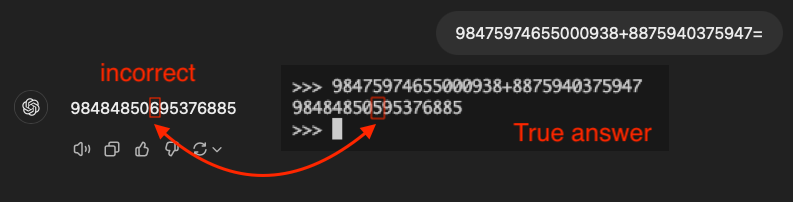
\includegraphics[width=0.9\textwidth]{fig/gpt4o_add_fail.png}
    \end{figure}
\end{frame}

\begin{frame}
    \frametitle{Motivation (cont.)}
    \begin{itemize}
        \item Why is this important?
        \item Maybe just guardrail models by hard-coding some rules?
        \item Not generally, because we would not train and use the models, if we could hard-code the rules in the first place.
        \item We want to understand the limitations of the models and improve them.
    \end{itemize}
\end{frame}

\begin{frame}
    \frametitle{Problem Statement}
    \begin{itemize}
        \item Focus on standard decoder-only transformers with absolute positional encodings.
        \item Try to improve generalization without altering model architecture or task-specific modifications.
        \item Explore data formatting and training data diversity.
    \end{itemize}
\end{frame}

\begin{frame}
    \frametitle{Research Questions}
    \begin{enumerate}
        \item Why do transformers with absolute positional encodings fail to generalize integer addition to longer sequences?
        \item How does the inclusion of sub-task data influence the model's compositionality and length generalization capabilities?
    \end{enumerate}
\end{frame}

\section{Background}

\begin{frame}
    \frametitle{Transformers}
    \begin{columns}
        \begin{column}{0.6\textwidth}
            \begin{itemize}
                \item Utilize self-attention to process sequential data.
                \item Focus on decoder-only models (b).
                \item Capable of capturing long-range dependencies without recurrence.
            \end{itemize}
        \end{column}
        \begin{column}{0.4\textwidth}
            \begin{figure}
                \centering
                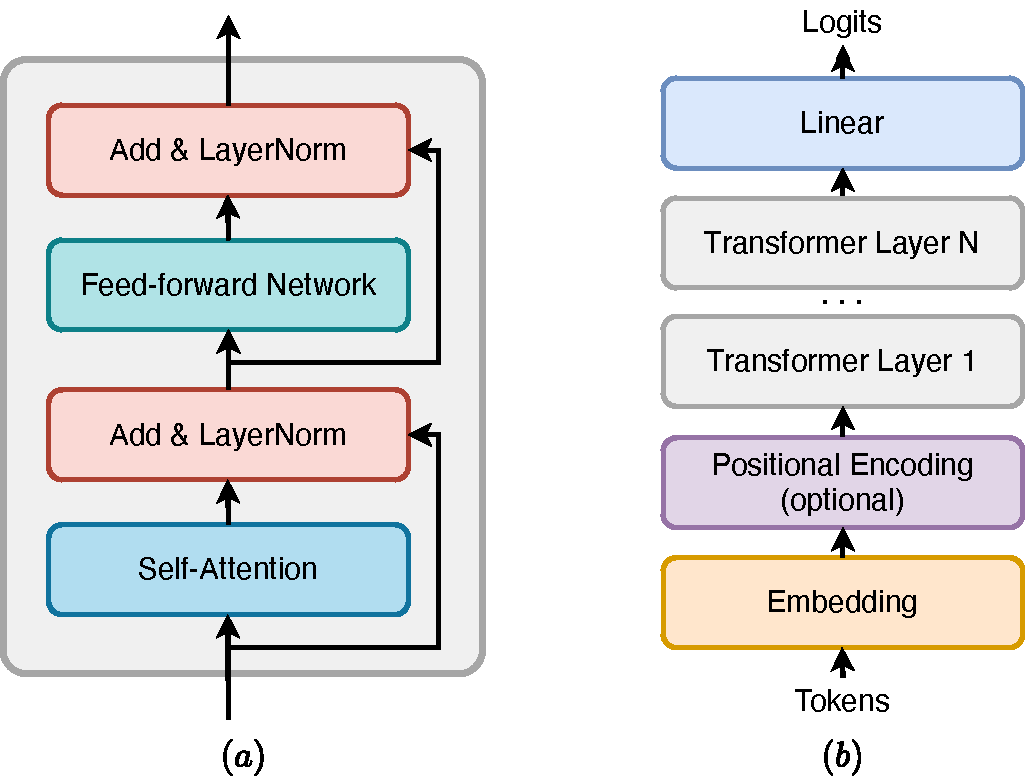
\includegraphics[width=\textwidth]{fig/transformer_layer.pdf}
            \end{figure}
        \end{column}
    \end{columns}
\end{frame}

\begin{frame}
    \frametitle{Positional Encodings (PE)}
    \begin{itemize}
        \item No explicit positional awareness in transformers.
        \item PEs inject sequence order information.
        \item Can be absolute or relative.
              \begin{itemize}
                  \item Absolute PEs: \\ \texttt{0, 1, 2, 3, ...}
                  \item Relative PEs: \\ \texttt{..., -3, -2, -1, 0, 1, 2, 3, ...}
              \end{itemize}
    \end{itemize}
\end{frame}

\begin{frame}
    \frametitle{Absolute Positional Encoding}
    \begin{itemize}
        \item Adds fixed positional information to input embeddings.
        \item Sinusoidal absolute PEs introduced by Vaswani et al. (2017):
              \[
                  \begin{aligned}
                      \text{PE}_{(pos, 2i)}   & = \sin\left( \frac{pos}{10000^{2i / d_{\text{model}}}} \right) \\
                      \text{PE}_{(pos, 2i+1)} & = \cos\left( \frac{pos}{10000^{2i / d_{\text{model}}}} \right)
                  \end{aligned}
              \]
    \end{itemize}
\end{frame}

\section{Related Work}
\begin{frame}
    \frametitle{Challenges in Length Generalization}
    \begin{itemize}
        \item Easy to grok addition for in-distribution lengths.
        \item Transformers struggle with sequences longer than seen in training.
        \item Addition requires accurate \emph{digit alignment} for all lengths.
        \item Positional encodings are crucial for digit alignment.
    \end{itemize}
\end{frame}

\begin{frame}
    \frametitle{Issues with Positional Encodings}
    \begin{itemize}
        \item Models struggle to select relevant tokens based on position in longer sequences.
        \item Failure to align digits without explicit positional cues.
        \item Research focuses on easing digit alignment.
    \end{itemize}
\end{frame}

\begin{frame}
    \frametitle{Improving Length Generalization}
    \begin{itemize}
        \item Reversing answer and training with scratchpad (Lee et al. 2024).
        \item Randomized PEs (Ruoss et al. 2023).
        \item Random spaces and scratchpad (Shen et al. 2023).
        \item Index hints \texttt{a1b2c3+a4b5c6=a5b7c9} (Y. Zhou et al. 2024)
        \item Task-specific PEs, e.g. Abacus (McLeish et al. 2024).
    \end{itemize}
\end{frame}

\begin{frame}
    \frametitle{Length Generalization Ratio}
    \begin{itemize}
        \item Ratio of the length of solved test problems to training lengths.
        \item 1x with data formatting (Lee et al. 2024).
        \item 1.1x with Random PE (Shen et al. 2023).
        \item 1.125x with NoPE (Kazemnejad et al. 2023).
        \item 1.5x with index hints and special setup (H. Zhou et al. 2023).
        \item 2.5x with FIRE and index hints (Y. Zhou et al. 2024).
        \item \textbf{6x} achieved with Abacus encoding (McLeish et al. 2024).
    \end{itemize}
\end{frame}

\begin{frame}
    \frametitle{SOTA: Abacus Encoding}
    \begin{itemize}
        \item Encode digit position relative to the start of the number.
        \item Task specific and requires reversing numbers.
        \item Use sinusoidal PE with indices specified by the Abacus encoding.
        \item Combined with architectural modifications like input injection and recurrent layers.
        \item Trained on up to 20 digits, generalizes to 120 digits.
    \end{itemize}
    \begin{figure}
        \centering
        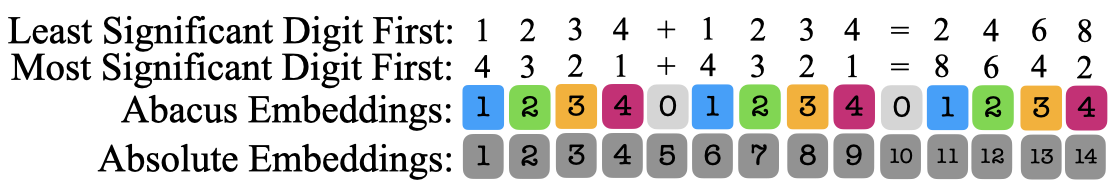
\includegraphics[width=0.7\textwidth]{fig/abacus.png}
        \caption{Source: McLeish et al. 2024}
    \end{figure}
\end{frame}

\begin{frame}
    \frametitle{Conclusions from Related Work}
    \begin{itemize}
        \item No common dataset $\rightarrow$ hard to compare methods.
        \item Positional encodings and data formatting significantly impact length generalization.
        \item Task-specific design can boost generalization to unseen lengths.
        \item Some diverge from standard decoder unsupervised training.
    \end{itemize}
\end{frame}

\begin{frame}
    \frametitle{Limitations of Existing Methods}
    \begin{itemize}
        \item Some successful methods lose sight of the original task:\\
              It's not about addition, but about model capabilities.
        \item Task-specific modifications are not always feasible.
        \item For the same reason e.g. index hints or scratchpad are "hacky."
        \item No common benchmark datasets or setups.
        \item Desire for simpler methods without altering model architecture.
    \end{itemize}
\end{frame}

\section{Approach}

\begin{frame}
    \frametitle{Overview of Approach}
    \begin{itemize}
        \item Baseline performance (Lee et al. 2023).
        \item Fixed positional patterns in absolute PE.
        \item Length generalization with different data formats.
        \item Weak generalization by breaking positional patterns.
        \item Sub-task data to improve compositionality.
    \end{itemize}
\end{frame}

\begin{frame}
    \frametitle{Baseline with Absolute Positional Encoding}
    \begin{itemize}
        \item High accuracy on training lengths (1 and 3 digits).
        \item No generalization on unseen lengths (2 and 4 digits).
    \end{itemize}
    \begin{figure}
        \centering
        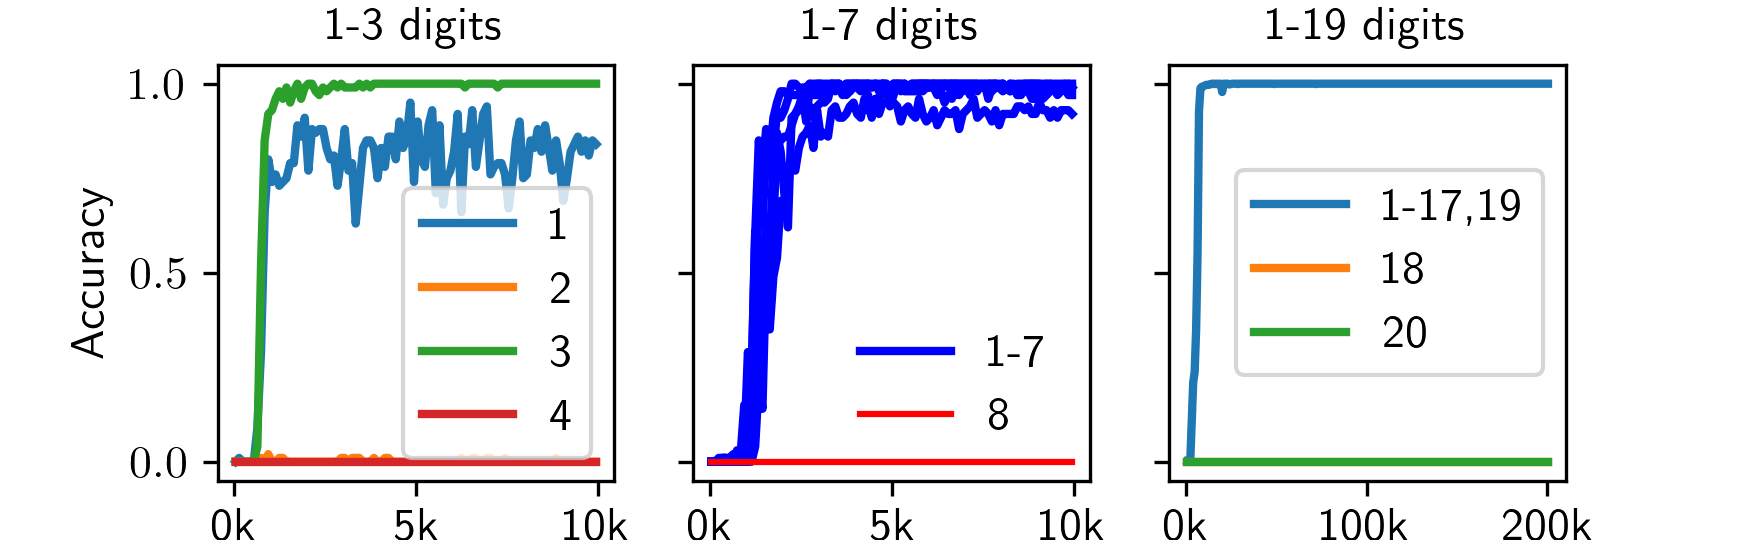
\includegraphics[width=0.85\textwidth]{fig/baseline_and_longer.png}
    \end{figure}
\end{frame}

\begin{frame}
    \frametitle{Next-Token Uncertainty Analysis}
    \begin{figure}
        \centering
        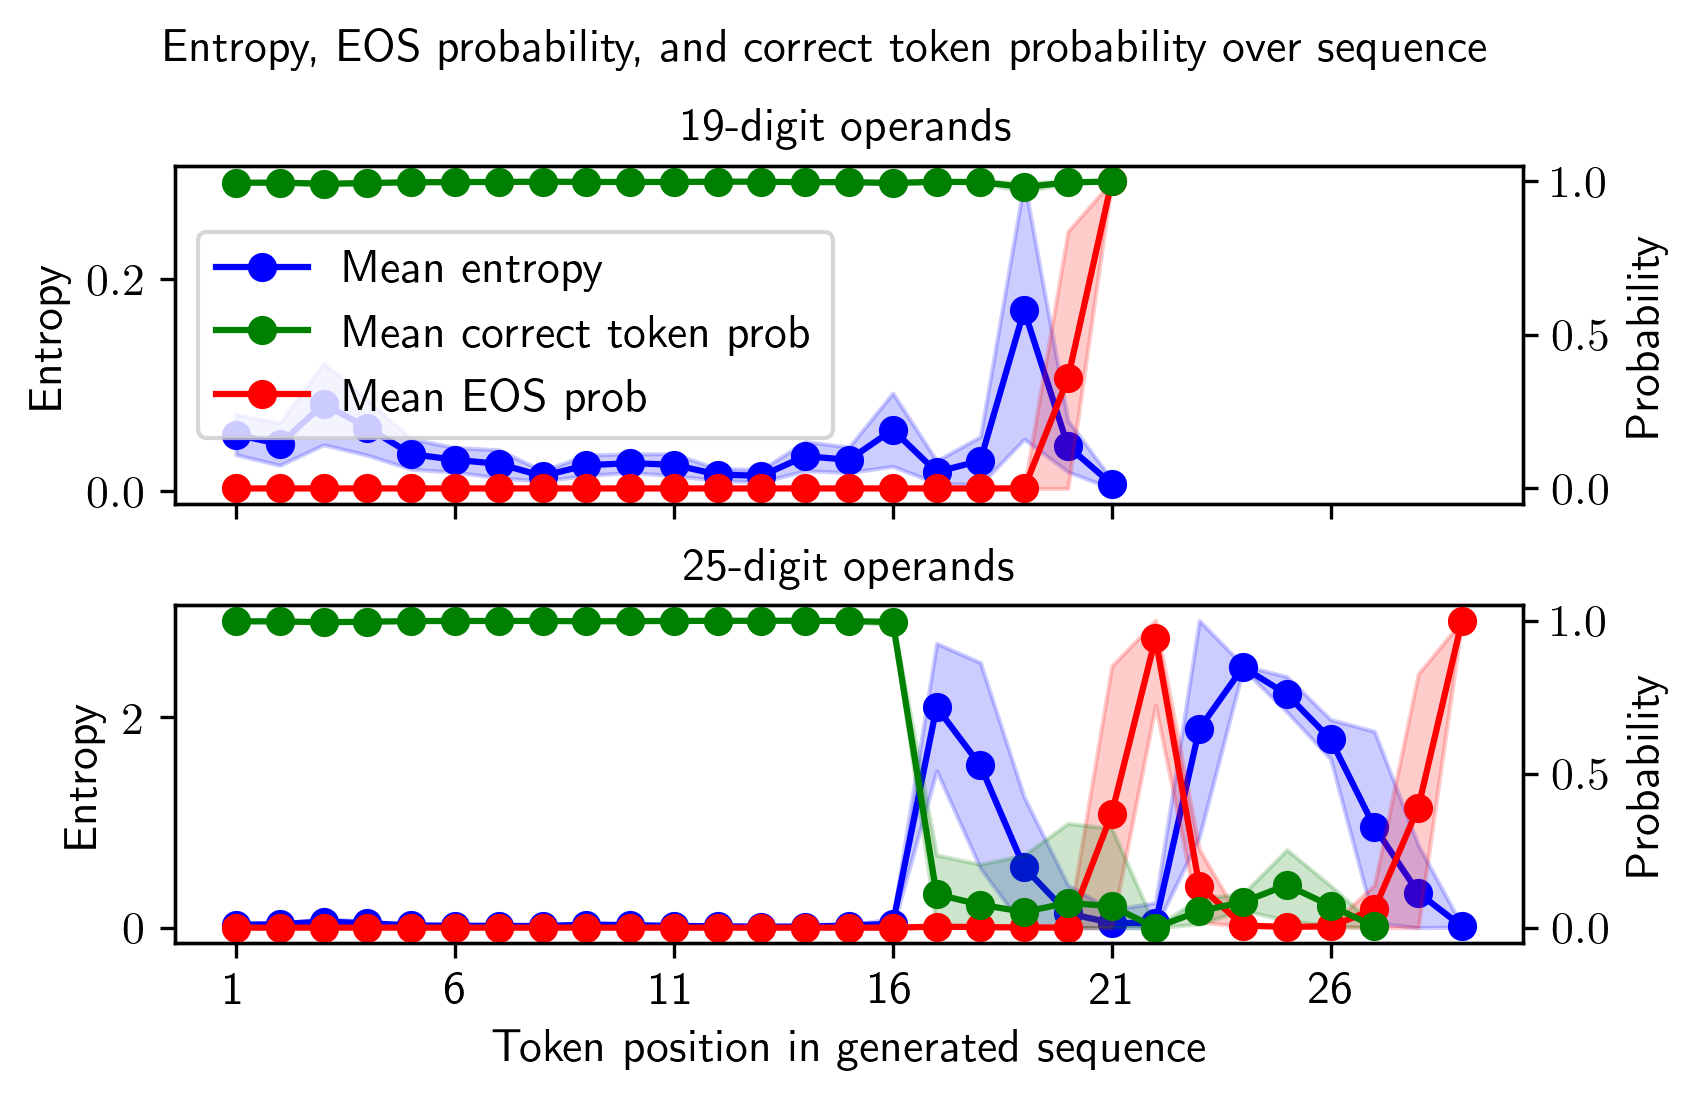
\includegraphics[width=0.65\linewidth]{fig/next_token_entropy.png}
    \end{figure}
\end{frame}

\begin{frame}
    \frametitle{Next-Token Uncertainty Analysis}
    \begin{itemize}
        \item For in-distribution lengths (1--17 and 19), models are confident in predictions (low entropy)
        \item For any OOD lengths (18 and 20+), entropy increases and model becomes uncertain.
        \item Next-token distribution $\approx$uniform for extreme OOD lengths.
        \item Predictions are not ``confident and wrong'' but ``uncertain and wrong.''
        \item Indicates that learned algorithm ``hardcodes'' positional patterns.
    \end{itemize}
\end{frame}

\begin{frame}
    \frametitle{Limitations of Absolute Positional Encoding}
    \begin{itemize}
        \item No generalization to unseen lengths.
        \item Neither in-between lengths (e.g. 18) nor longer lengths (20+).
        \item Learned algorithm completely breaks for OOD lengths.
        \item Literature suggests aligning digits is the key challenge.
        \item Next: try to break positional patterns with data formatting.
    \end{itemize}
\end{frame}

\begin{frame}
    \frametitle{Data Formatting Techniques}
    \begin{itemize}
        \item Standard Format \\
              \texttt{\$123+456=579\$}
        \item Zero Padding \\
              \texttt{\$00123+00456=00579\$} ($N_{\text{pad}} = 5$)
        \item Reversing \\
              \texttt{\$321+654=975\$}
        \item Random Spaces \\
              \texttt{\$1 23 +4  5 6=579\$}
        \item Scratchpad \\
              \texttt{\$567+789=7 6 5 + 9 8 7;
                  c=0,7+0+0=7,c=0;
                  6+9+0=5,c=1;
                  5+8+1=4,c=1;
                  0+7+1=8,c=0|8457\$}
    \end{itemize}
\end{frame}

\begin{frame}
    \frametitle{Data Formatting Results}
    \begin{figure}
        \centering
        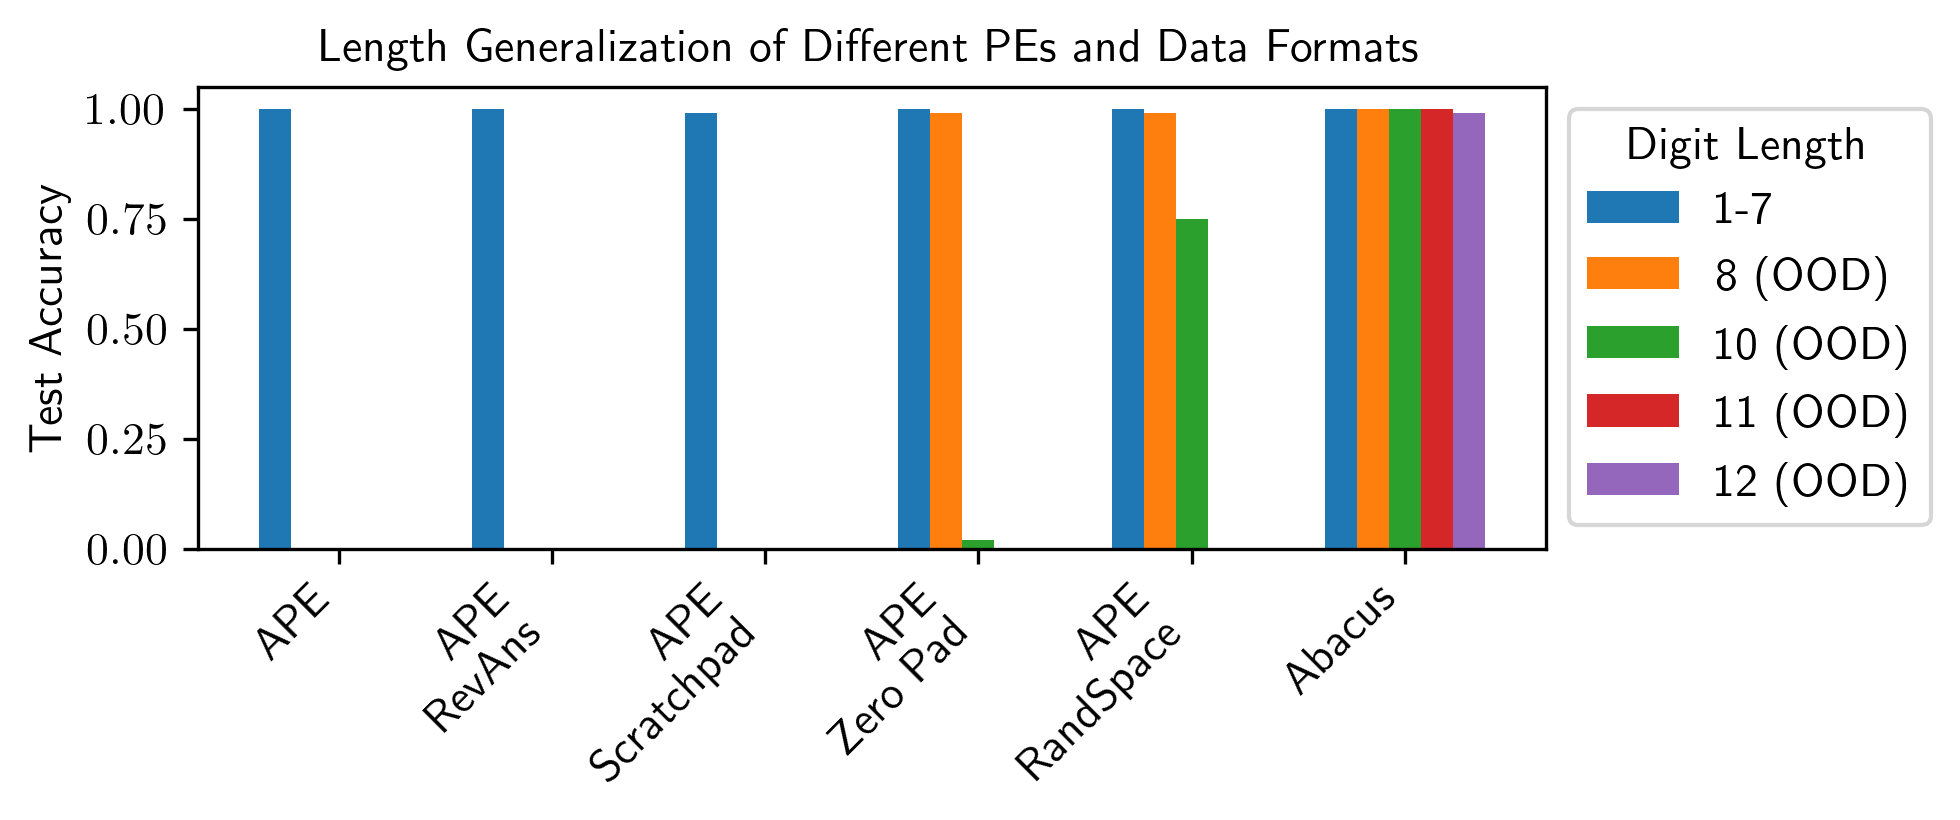
\includegraphics[width=0.85\linewidth]{fig/pe_results.png}
    \end{figure}
\end{frame}

\begin{frame}
    \frametitle{Data Formats Summary}
    \begin{itemize}
        \item Zero padding can ``close the gap'' in OOD lengths (7, \textbf{8}, 9 digits).
        \item Random spaces weakly improve generalization (x1.125).
        \item Other methods do not help generalization.
        \item Random spaces smooth attention patterns.
        \item Abacus generalizes well.
    \end{itemize}
\end{frame}

\begin{frame}
    \frametitle{Sub-tasks for Compositionality}
    \begin{itemize}
        \item A different direction to improve generalization.
        \item Encourage model to learn an \emph{algorithm}.
        \item Include \emph{sub-task} data in training.
        \item Sub-tasks can be composed to perform addition.
    \end{itemize}
\end{frame}

\begin{frame}
    \frametitle{Sub-task Data}
    \begin{itemize}
        \item Parts of the addition process broken down into sub-tasks.
        \item Sub-tasks include:
              \begin{itemize}
                  \item Digit Alignment
                  \item Reversing
                  \item Carry Detection
                  \item Digit-wise Modular Addition
                  \item Addition
              \end{itemize}
        \item Each sub-task has a specific format.
        \item Add a prefix to the input sequence to indicate the sub-task.
              \texttt{\$pre123+456=}
    \end{itemize}
\end{frame}

\begin{frame}
    \frametitle{Experiment Setup}
    \begin{itemize}
        \item 1-7 digits in-distribution, 8 and 10 digits OOD.
        \item Model dimension: 64--1536 (increments of 64).
        \item Dataset sizes: 10K, 100K, 1M, 10M samples.
        \item Addition-only and mixed-task for each.
        \item 3 seeds per run.
    \end{itemize}
\end{frame}

\begin{frame}
    \frametitle{Impact of Sub-task Learning}
    \begin{table}
        \centering
        \begin{tabular}{lccccc}
            \toprule
                    & \multicolumn{2}{c}{8 Digits} & \multicolumn{2}{c}{10 Digits}                                          \\
            Dataset & Add                          & Mix                           & Add   & Mix           & Diff           \\
            \midrule
            10K     & 7.0 ± 22.7                   & 35.4 ± 39.6                   & 0 ± 0 & 2.4 ± 8.4     & \textbf{+15.4} \\
            100K    & 21.5 ± 29.7                  & 41.8 ± 36.5                   & 0 ± 0 & 1.0 ± 5.2     & \textbf{+10.6} \\
            1M      & 16.1 ± 24.8                  & 39.5 ± 36.3                   & 0 ± 0 & 1.5 ± 7.6     & \textbf{+12.4} \\
            10M     & 18.6 ± 33.1                  & 37.3 ± 37.2                   & 0 ± 0 & 3.1 ± 10.1    & \textbf{+10.9} \\
            \midrule
            Diff    &                              & \textbf{+22.7}                &       & \textbf{+2.0} &                \\
            \bottomrule
        \end{tabular}
    \end{table}
\end{frame}

\begin{frame}
    \frametitle{Test Loss vs. Model Dimension}
    \begin{figure}
        \centering
        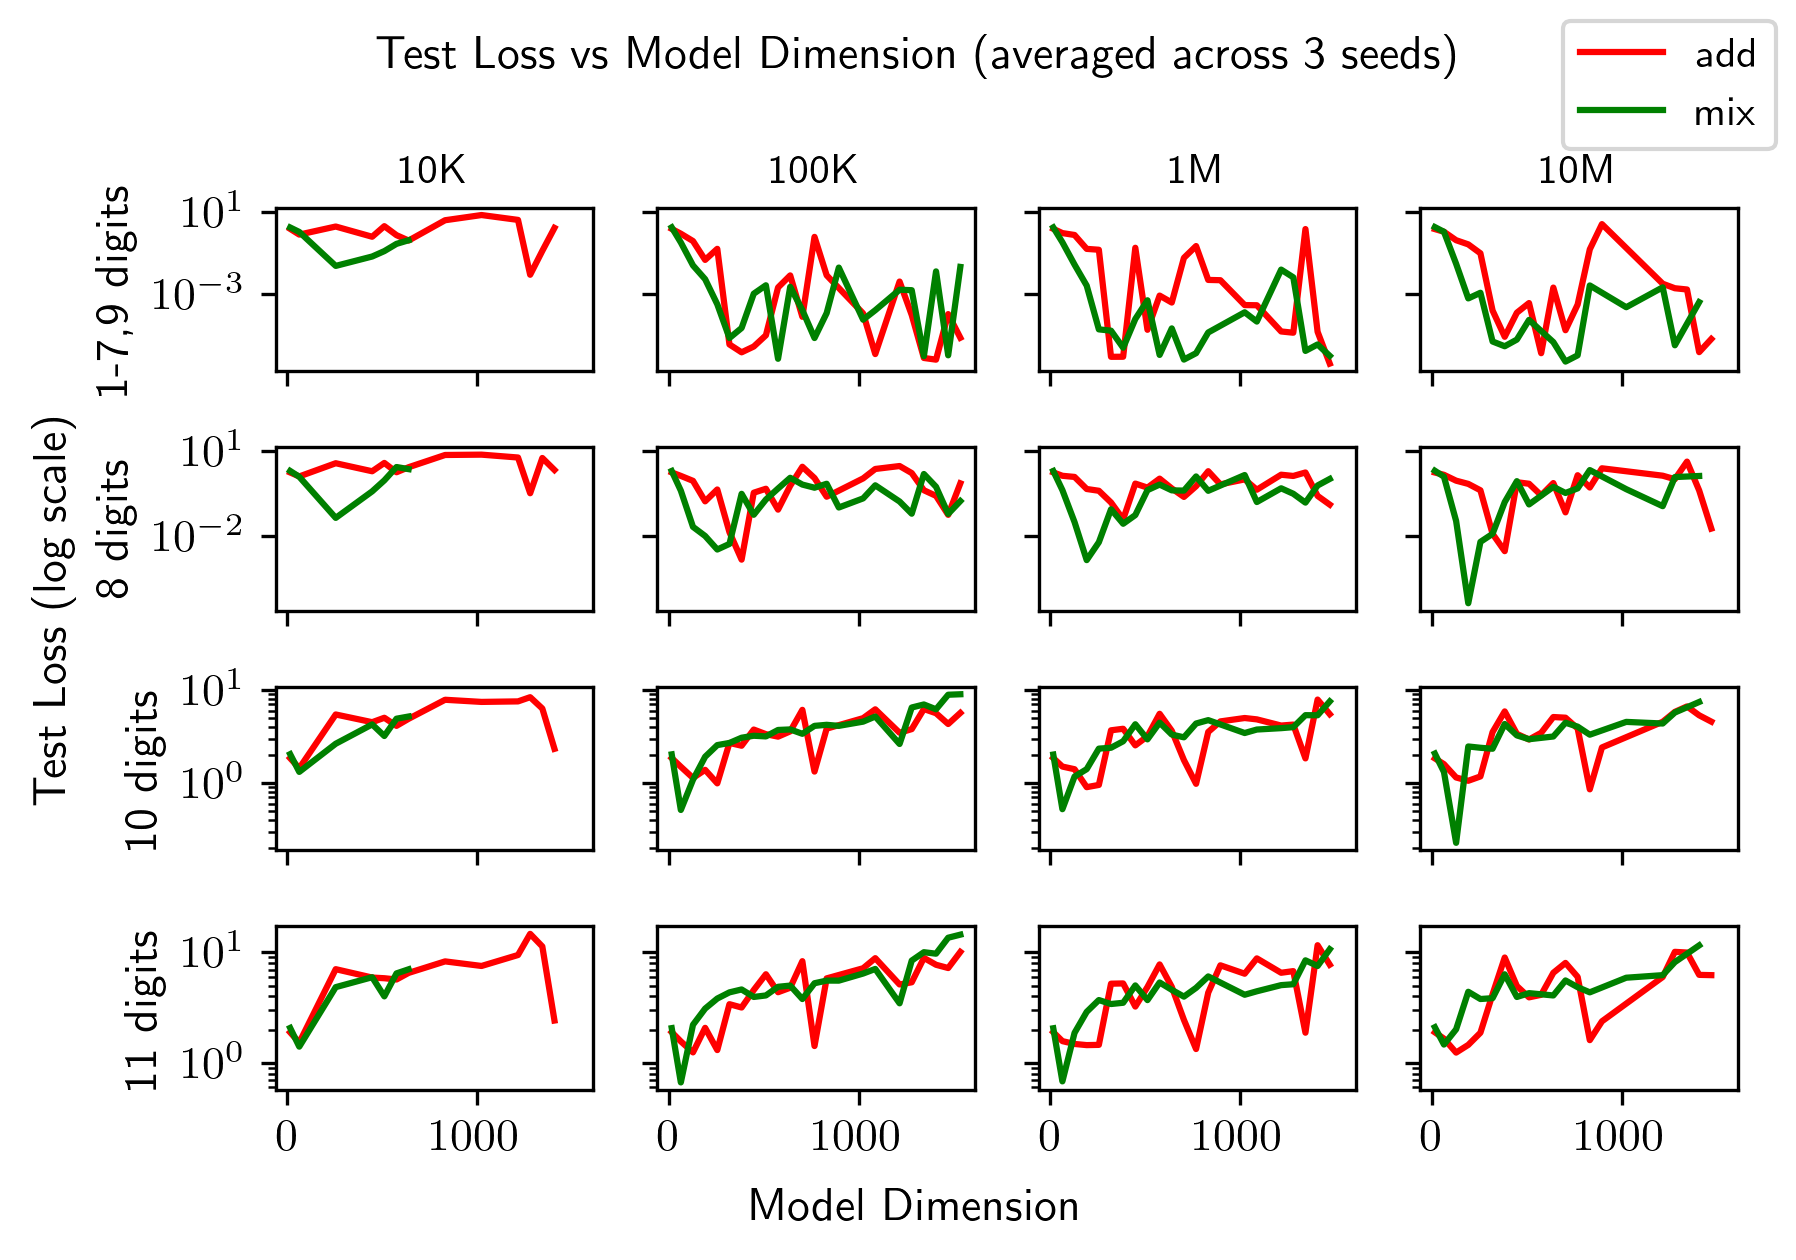
\includegraphics[width=0.6\linewidth]{fig/exp_27_test_loss_vs_n_embd.png}
    \end{figure}
\end{frame}

\begin{frame}
    \frametitle{Test Loss vs. Model Dimension}
    \begin{itemize}
        \item Smaller models benefit more from mixed-task training.
        \item Effect diminishes as model size increases.
        \item Mixed-task training never hurts performance.
    \end{itemize}
\end{frame}

\begin{frame}
    \frametitle{In-Distribution vs. OOD Test Loss}
    \begin{figure}
        \centering
        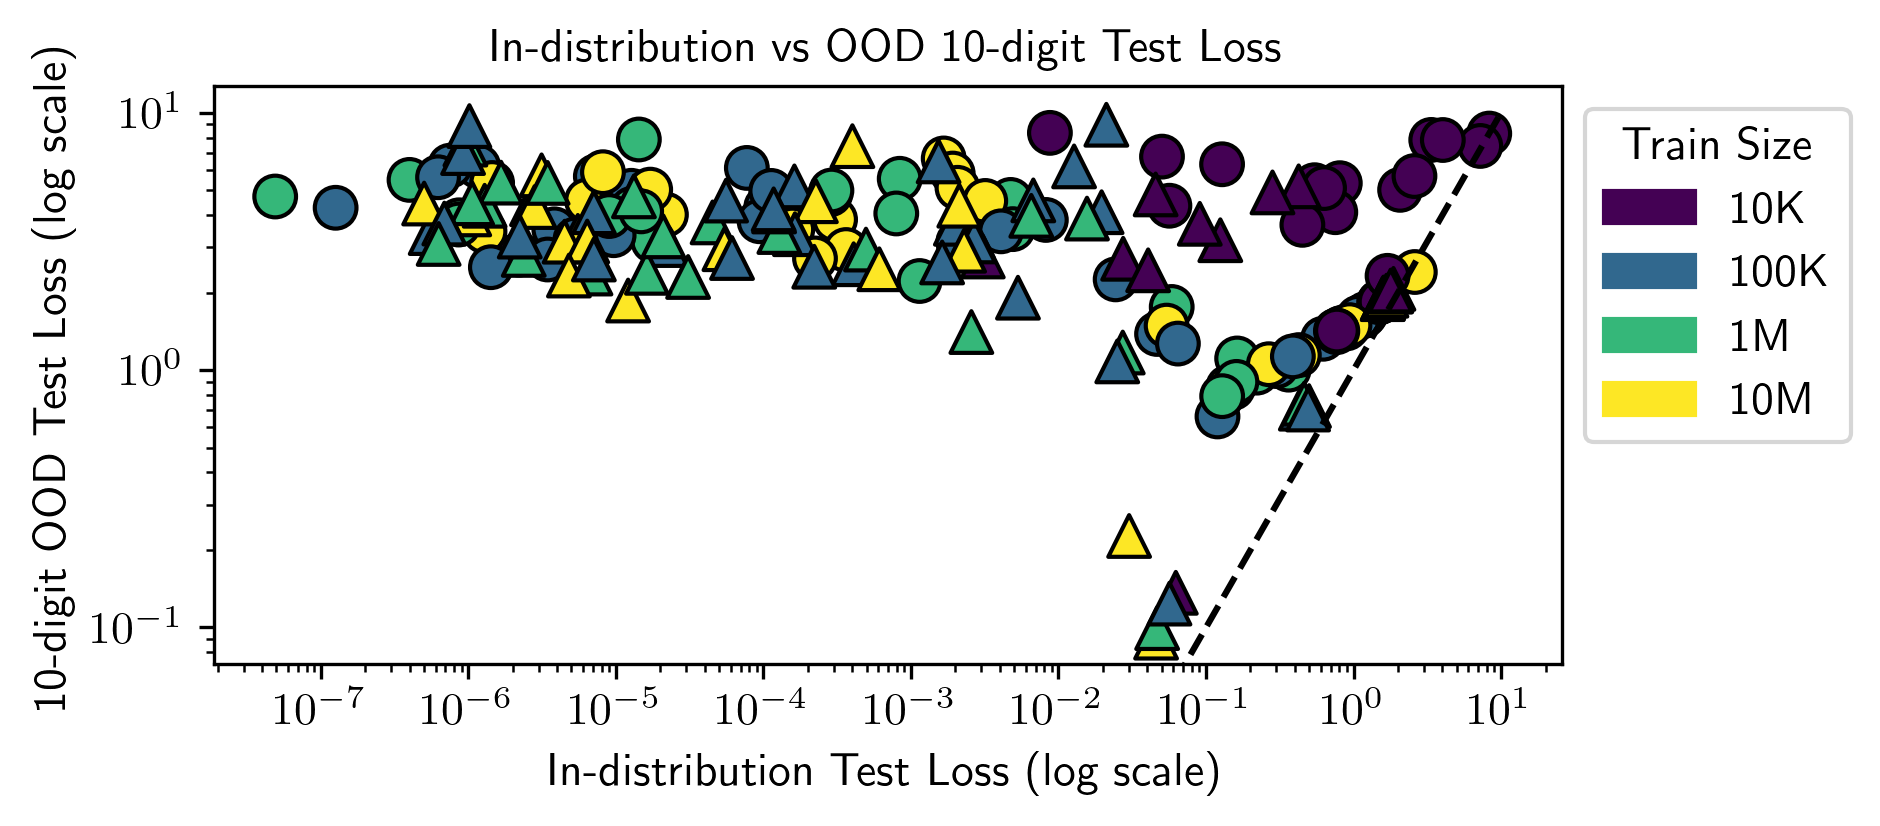
\includegraphics[width=0.8\linewidth]{fig/subtask_overfitting.png}
    \end{figure}
\end{frame}


\begin{frame}
    \frametitle{In-Distribution vs. OOD Test Loss}
    \begin{itemize}
        \item Mixed-task can be a Pareto-improvement.
        \item Allows to reduce OOD loss without increasing in-distribution loss.
    \end{itemize}
\end{frame}


\section{Conclusion}

\begin{frame}
    \frametitle{Summary of Findings}
    \begin{itemize}
        \item Absolute positional encodings fail to generalize.
        \item Generalization possible without architecture changes.
        \item Random spaces can improve generalization.
        \item Sub-task data improves generalization, especially for smaller models and datasets.
    \end{itemize}
\end{frame}

\begin{frame}
    \frametitle{Limitations}
    \begin{itemize}
        \item Focused on small models trained from scratch; applicability to large language models (LLMs) is unclear.
        \item Other positional encodings were not explored; alternative solutions might exist.
        \item Sub-task experiments may be under-trained due to limited training steps.
        \item Lack of mechanistic interpretability.
    \end{itemize}
\end{frame}

\begin{frame}
    \frametitle{Future Work}
    \begin{itemize}
        \item Develop mechanistic interpretability methods for algorithmic tasks.
        \item Apply to fine-tuning pre-trained LLMs and data curation.
        \item Experiment more with smaller models for sub-task learning.
        \item Explore active learning and curriculum learning.
    \end{itemize}
\end{frame}

\begin{frame}
    \frametitle{Questions}
    \centering
    Thank you for your attention! \\
    \vspace{1cm}
    Questions?
\end{frame}


\begin{frame}[allowframebreaks]
    \frametitle{References}
    \scriptsize
    \begin{thebibliography}{}
        \bibitem{lee2023}
        Lee, N., Sreenivasan, K., Lee, J., Lee, K., \& Papailiopoulos, D. (2023). \emph{Teaching Arithmetic to Small Transformers}.
        The 3rd Workshop on Mathematical Reasoning and AI at NeurIPS'23.

        \bibitem{kazemnejad2023}
        Kazemnejad, A., Padhi, I., Natesan, K., Das, P., \& Reddy, S. (2023). \emph{The Impact of Positional Encoding on Length Generalization in Transformers}.
        Thirty-seventh Conference on Neural Information Processing Systems.

        \bibitem{zhou2023}
        Zhou, H., Bradley, A., Littwin, E., Razin, N., Saremi, O., Susskind, J., Bengio, S., \& Nakkiran, P. (2023). \emph{What Algorithms can Transformers Learn? A Study in Length Generalization}. \emph{arXiv:2310.16028}.

        \bibitem{vaswani2017}
        Vaswani, A., Shazeer, N., Parmar, N., Uszkoreit, J., Jones, L., Gomez, A. N., Kaiser, Ł., \& Polosukhin, I. (2017). \emph{Attention is All You Need}.
        Advances in Neural Information Processing Systems, 30

        \bibitem{zhou2024}
        Zhou, Y., Alon, U., Chen, X., Wang, X., Agarwal, R., \& Zhou, D. (2024). \emph{Transformers Can Achieve Length Generalization But Not Robustly}.
        \emph{arXiv:2402.09371}.

        \bibitem{ruoss2023}
        Ruoss, A., Delétang, G., Genewein, T., Grau-Moya, J., Csordás, R., Bennani, M., Legg, S., \& Veness, J. (2023). \emph{Randomized Positional Encodings Boost Length Generalization of Transformers}. \emph{arXiv:2305.16843}.

        \bibitem{mcleish2024}
        McLeish, S., Bansal, A., Stein, A., Jain, N., Kirchenbauer, J., Bartoldson, B. R., Kailkhura, B., Bhatele, A., Geiping, J., Schwarzschild, A., \& Goldstein, T. (2024). \emph{Transformers Can Do Arithmetic with the Right Embeddings}. \emph{arXiv:2405.17399}.

        \bibitem{shen2023}
        Shen, R., Bubeck, S., Eldan, R., Lee, Y. T., Li, Y., \& Zhang, Y. (2023). \emph{Positional Description Matters for Transformers Arithmetic}. \emph{arXiv:2311.14737}.
    \end{thebibliography}
\end{frame}



% Appendix

\section{Appendix}

\begin{frame}
    \frametitle{Appendix: Counting Failure}
    \begin{itemize}
        \item Example: SOTA model GPT-4o struggles with simple counting.
    \end{itemize}
    \begin{figure}
        \centering
        \begin{minipage}{0.55\textwidth}
            \centering
            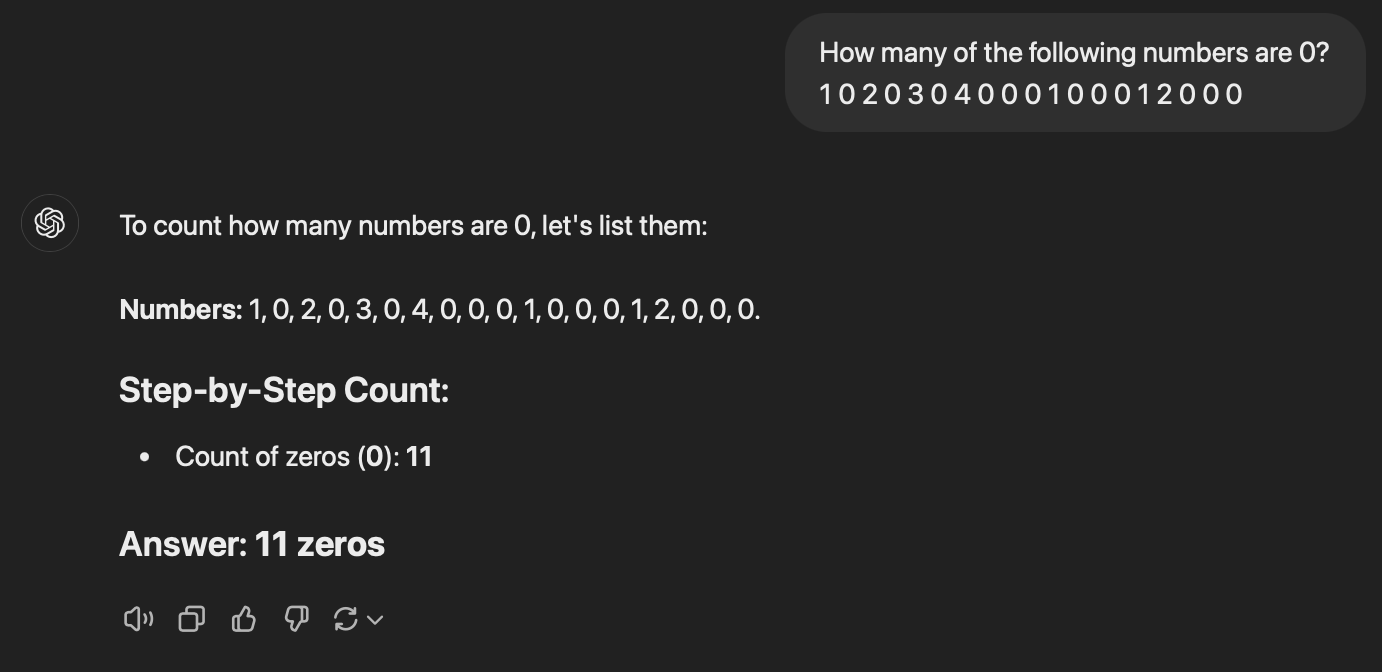
\includegraphics[width=\textwidth]{fig/gpt4o_count_fail.png}
        \end{minipage}
        \begin{minipage}{0.35\textwidth}
            \centering
            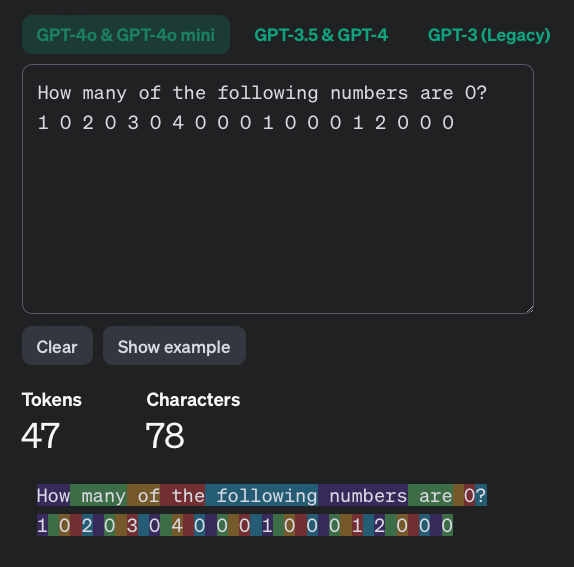
\includegraphics[width=\textwidth]{fig/gpt4o_count_fail_tokens.png}
        \end{minipage}
    \end{figure}
\end{frame}


\begin{frame}
    \frametitle{Appendix: Data Generation Process}
    \begin{itemize}
        \item Operands are randomly sampled positive integers
        \item Each operand has exactly the specified number of digits (no leading zeros)
        \item For digit lengths 1 to 3:
              \begin{itemize}
                  \item 1-digit operands: All 100 combinations (0 to 9)
                  \item 2-digit operands: 900 samples randomly selected
                  \item 3-digit operands: 9,000 samples randomly selected
              \end{itemize}
        \item For digit lengths 4 and above:
              \begin{itemize}
                  \item Equal number of samples per digit length to fill the dataset size
              \end{itemize}
        \item Test sets contain unique samples not present in the training set
    \end{itemize}
\end{frame}

\begin{frame}
    \frametitle{Appendix: Self-Attention Mechanism}
    \begin{itemize}
        \item Computes attention weights between all token pairs.
        \item Allows the model to focus on relevant parts of the sequence.
        \item Attention function:
              \[
                  \text{Attention}(Q, K, V) = \text{softmax}\left( \frac{Q K^\top}{\sqrt{d_k}} \right) V
              \]
        \item Where $Q$, $K$, $V$ are query, key, and value matrices.
    \end{itemize}
\end{frame}

\begin{frame}
    \frametitle{Appendix: Training and Inference}
    \begin{figure}
        \centering
        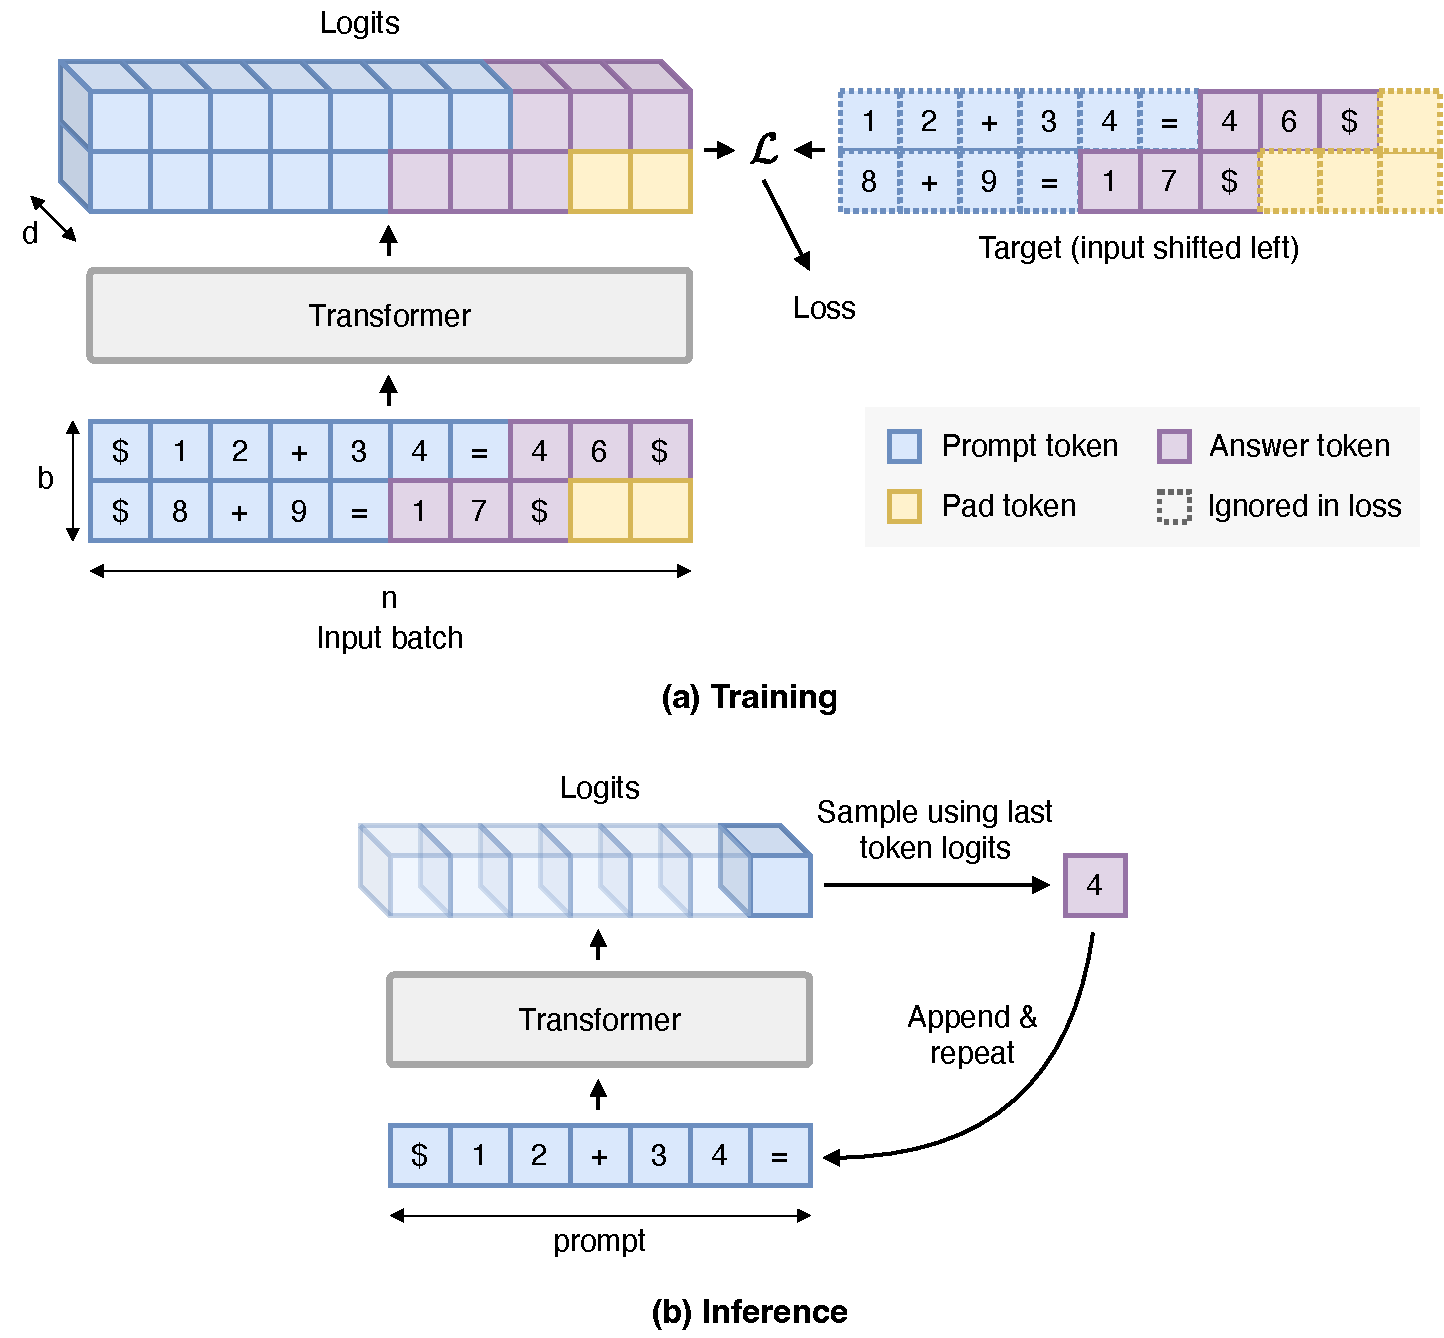
\includegraphics[width=0.45\textwidth]{fig/training_and_inference.pdf}
    \end{figure}
\end{frame}

\begin{frame}
    \frametitle{Attention Maps: Absolute PE}
    \begin{figure}
        \centering
        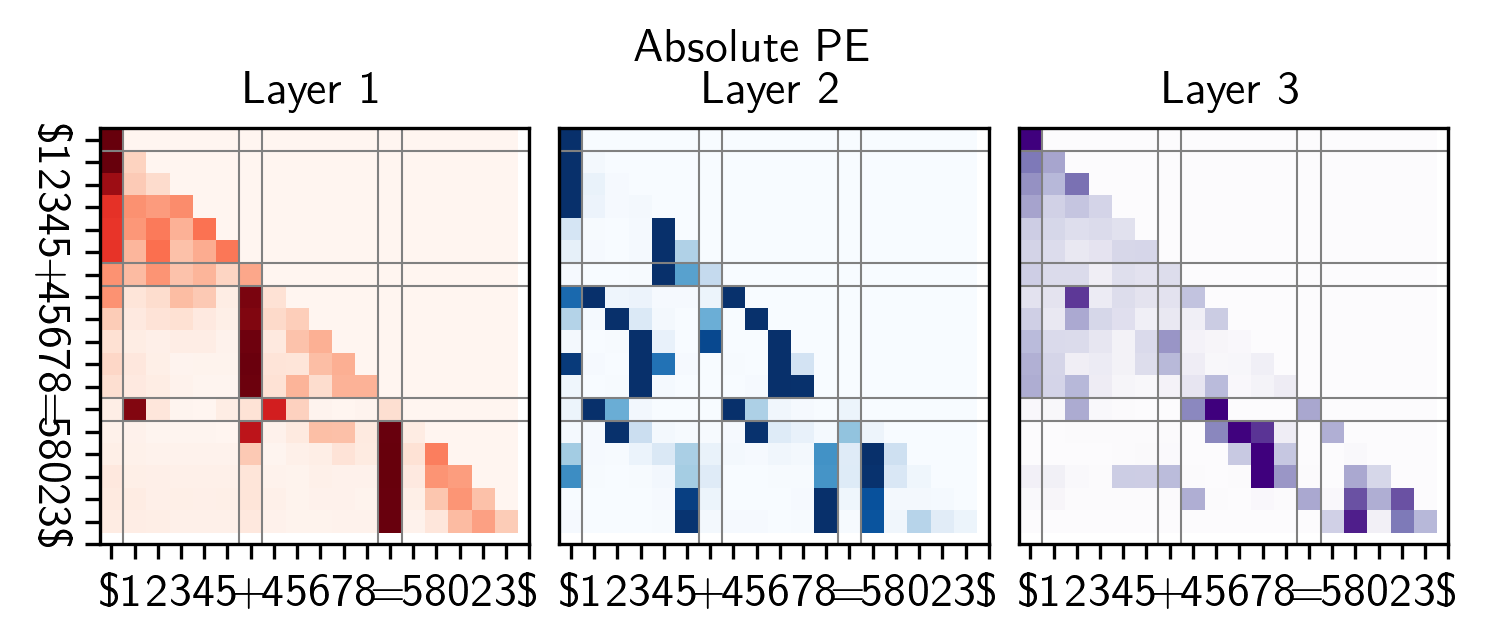
\includegraphics[width=0.9\linewidth]{fig/attn_map_abs_pe.png}
    \end{figure}
\end{frame}

\begin{frame}
    \frametitle{Attention Maps: Absolute PE with Random Spaces}
    \begin{figure}
        \centering
        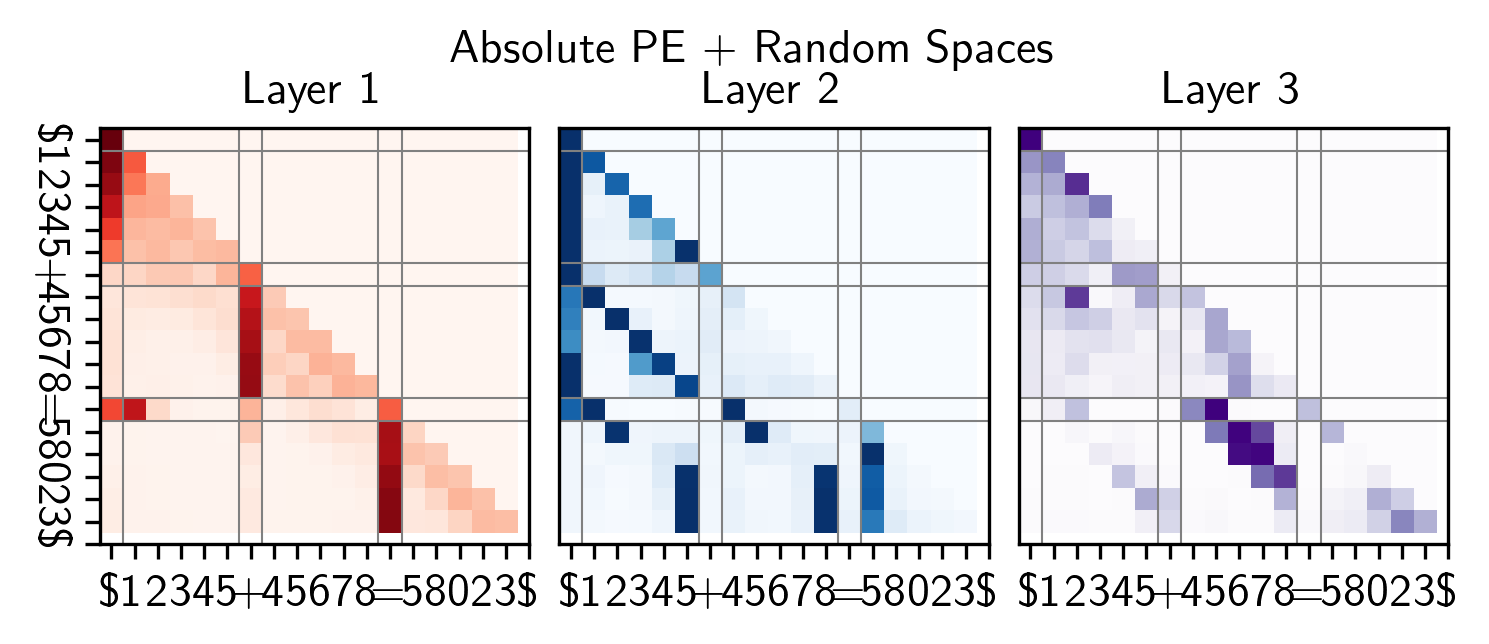
\includegraphics[width=0.9\linewidth]{fig/attn_map_abs_pe_random_spaces.png}
    \end{figure}
\end{frame}

\begin{frame}
    \frametitle{Attention Maps: Abacus PE}
    \begin{figure}
        \centering
        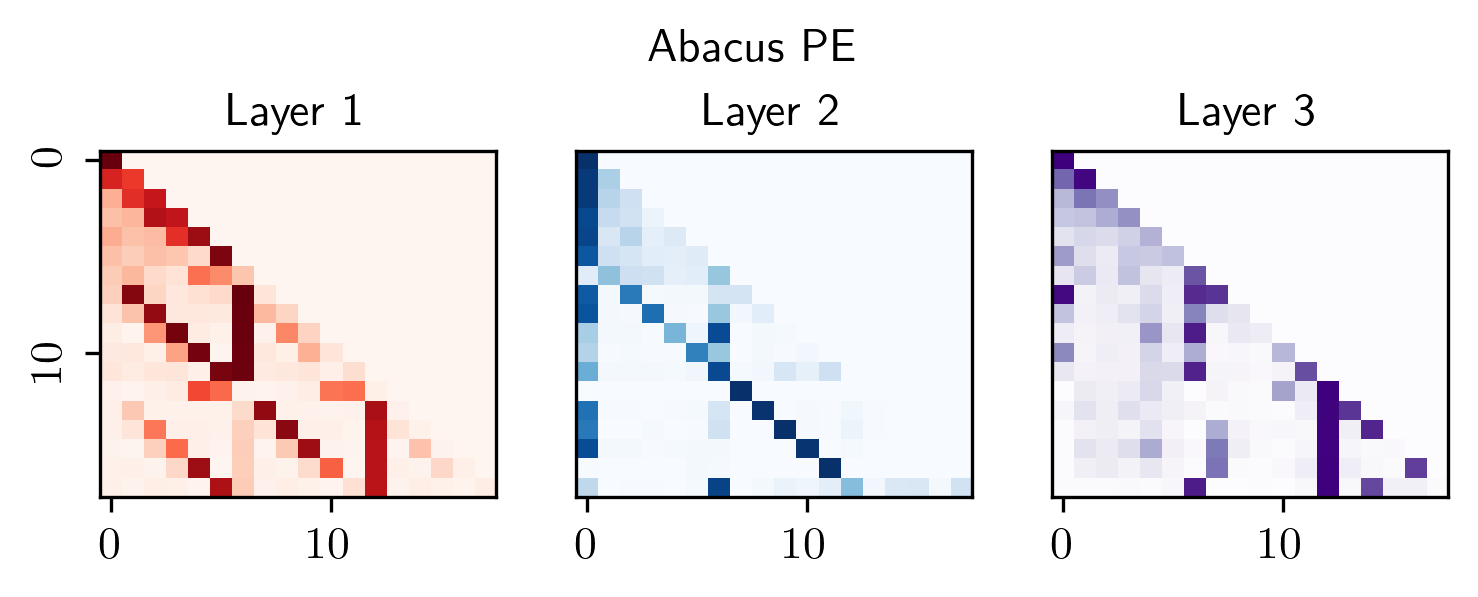
\includegraphics[width=0.9\linewidth]{fig/attn_map_abacus_pe.png}
    \end{figure}
\end{frame}

\begin{frame}
    \frametitle{Appendix: Scratchpad Evaluation}
    \begin{figure}
        \centering
        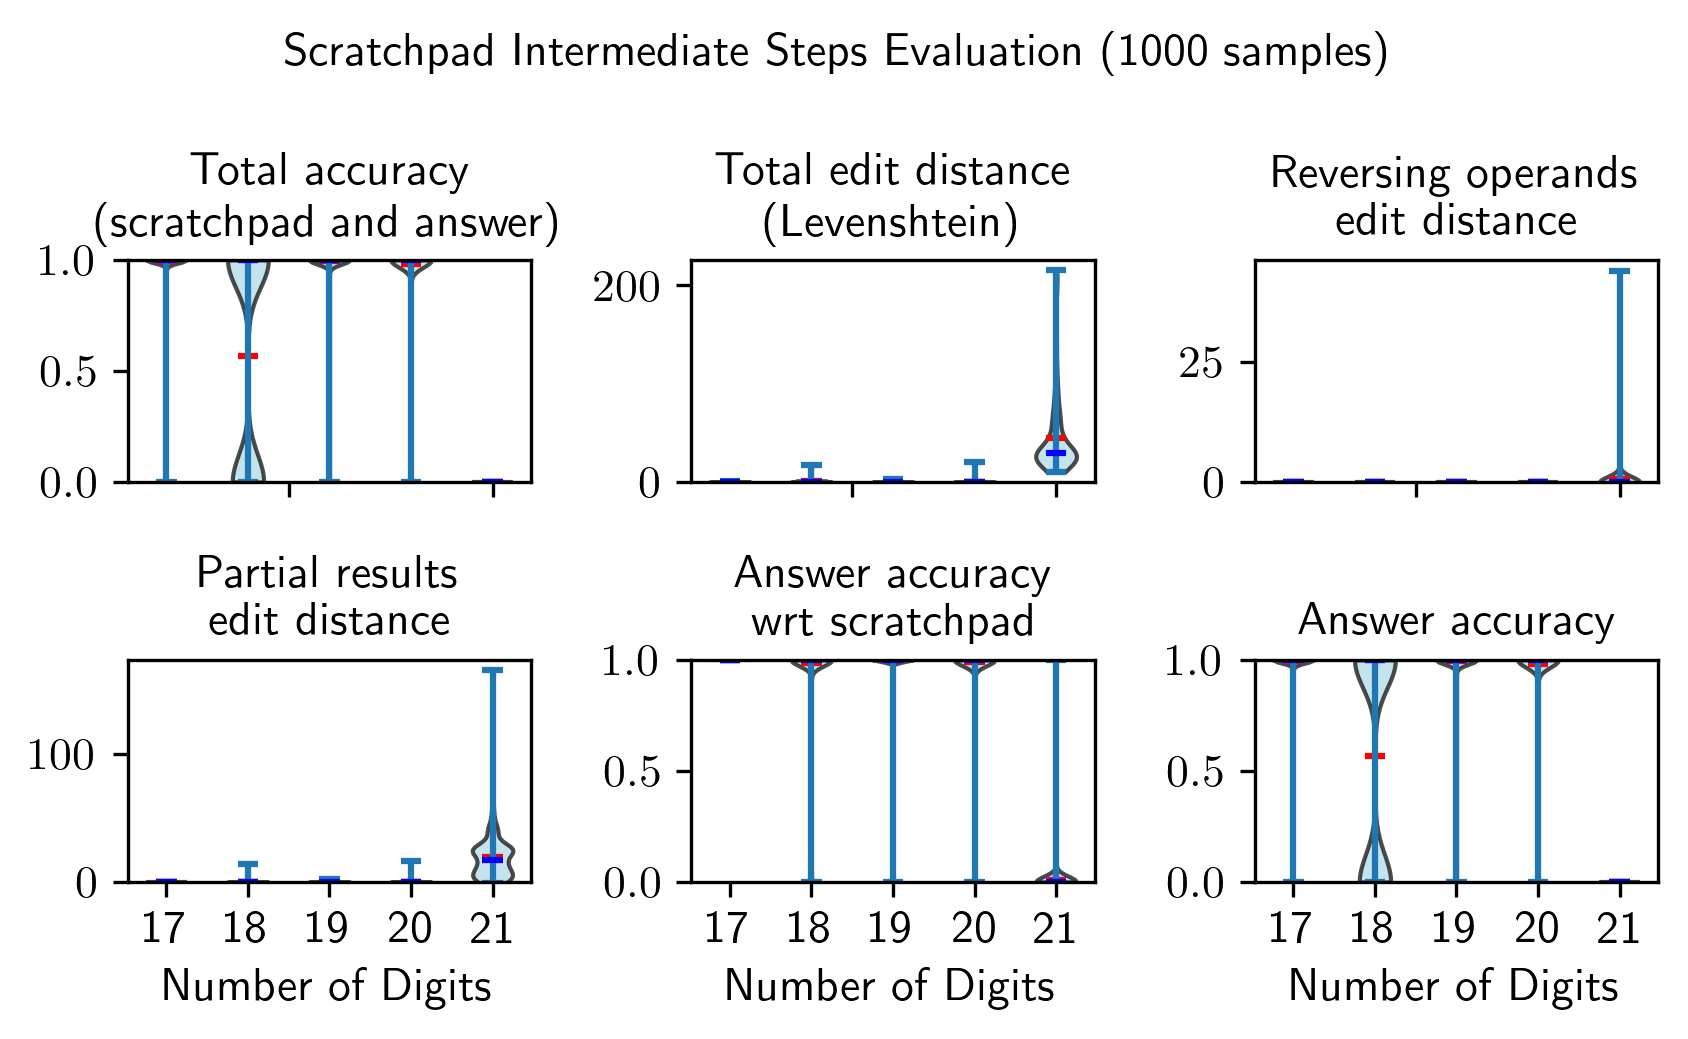
\includegraphics[width=0.6\linewidth]{fig/scratchpad_eval.png}
    \end{figure}
\end{frame}

\begin{frame}
    \frametitle{Appendix: Sub-task Prefix}
    \begin{itemize}
        \item Includes a 3-letter task prefix to differentiate sub-tasks
        \item Format: \texttt{xxx\$a+b=c\$}, where \texttt{xxx} is the sub-task identifier
    \end{itemize}
    \vspace{0.5em}
    \textbf{Example (Reversing sub-task):}
    \begin{center}
        \texttt{rev\$123+456=321+654\$}
    \end{center}
\end{frame}

\begin{frame}
    \frametitle{Appendix: Sub-task: Digit Alignment (\texttt{ali})}
    \begin{itemize}
        \item Focuses on aligning digits of the operands
        \item Model outputs corresponding digit pairs from each operand
    \end{itemize}
    \vspace{0.5em}
    \textbf{Example:}
    \begin{center}
        \texttt{ali\$1234+4567=1+4,2+5,3+6,4+7\$}
    \end{center}
\end{frame}

\begin{frame}
    \frametitle{Appendix: Sub-task: Reversing (\texttt{rev})}
    \begin{itemize}
        \item Involves reversing the digits of each operand
        \item Helps model understand the reversal operation
    \end{itemize}
    \vspace{0.5em}
    \textbf{Example:}
    \begin{center}
        \texttt{rev\$1234+4567=4321+7654\$}
    \end{center}
\end{frame}

\begin{frame}
    \frametitle{Appendix: Sub-task: Carry Detection (\texttt{car})}
    \begin{itemize}
        \item Model identifies positions where a carry operation occurs
        \item Output is a string of 'c's and dashes indicating carries
    \end{itemize}
    \vspace{0.5em}
    \textbf{Example:}
    \begin{center}
        \texttt{car\$1234+4567=---c\$}
    \end{center}
\end{frame}

\begin{frame}
    \frametitle{Appendix: Sub-task: Modular Addition (\texttt{mad})}
    \begin{itemize}
        \item Model performs addition modulo 10 on each pair of corresponding digits
        \item Does not consider carries
    \end{itemize}
    \vspace{0.5em}
    \textbf{Example:}
    \begin{center}
        \texttt{mad\$1234+4567=5791\$}
    \end{center}
\end{frame}

\begin{frame}
    \frametitle{Appendix: Sub-task: Addition (\texttt{add})}
    \begin{itemize}
        \item Standard addition task
        \item Model computes the sum of the two operands
    \end{itemize}
    \vspace{0.5em}
    \textbf{Example:}
    \begin{center}
        \texttt{add\$1234+4567=5801\$}
    \end{center}
\end{frame}

\begin{frame}
    \frametitle{Sub-task Difficulty Analysis}
    \begin{figure}
        \centering
        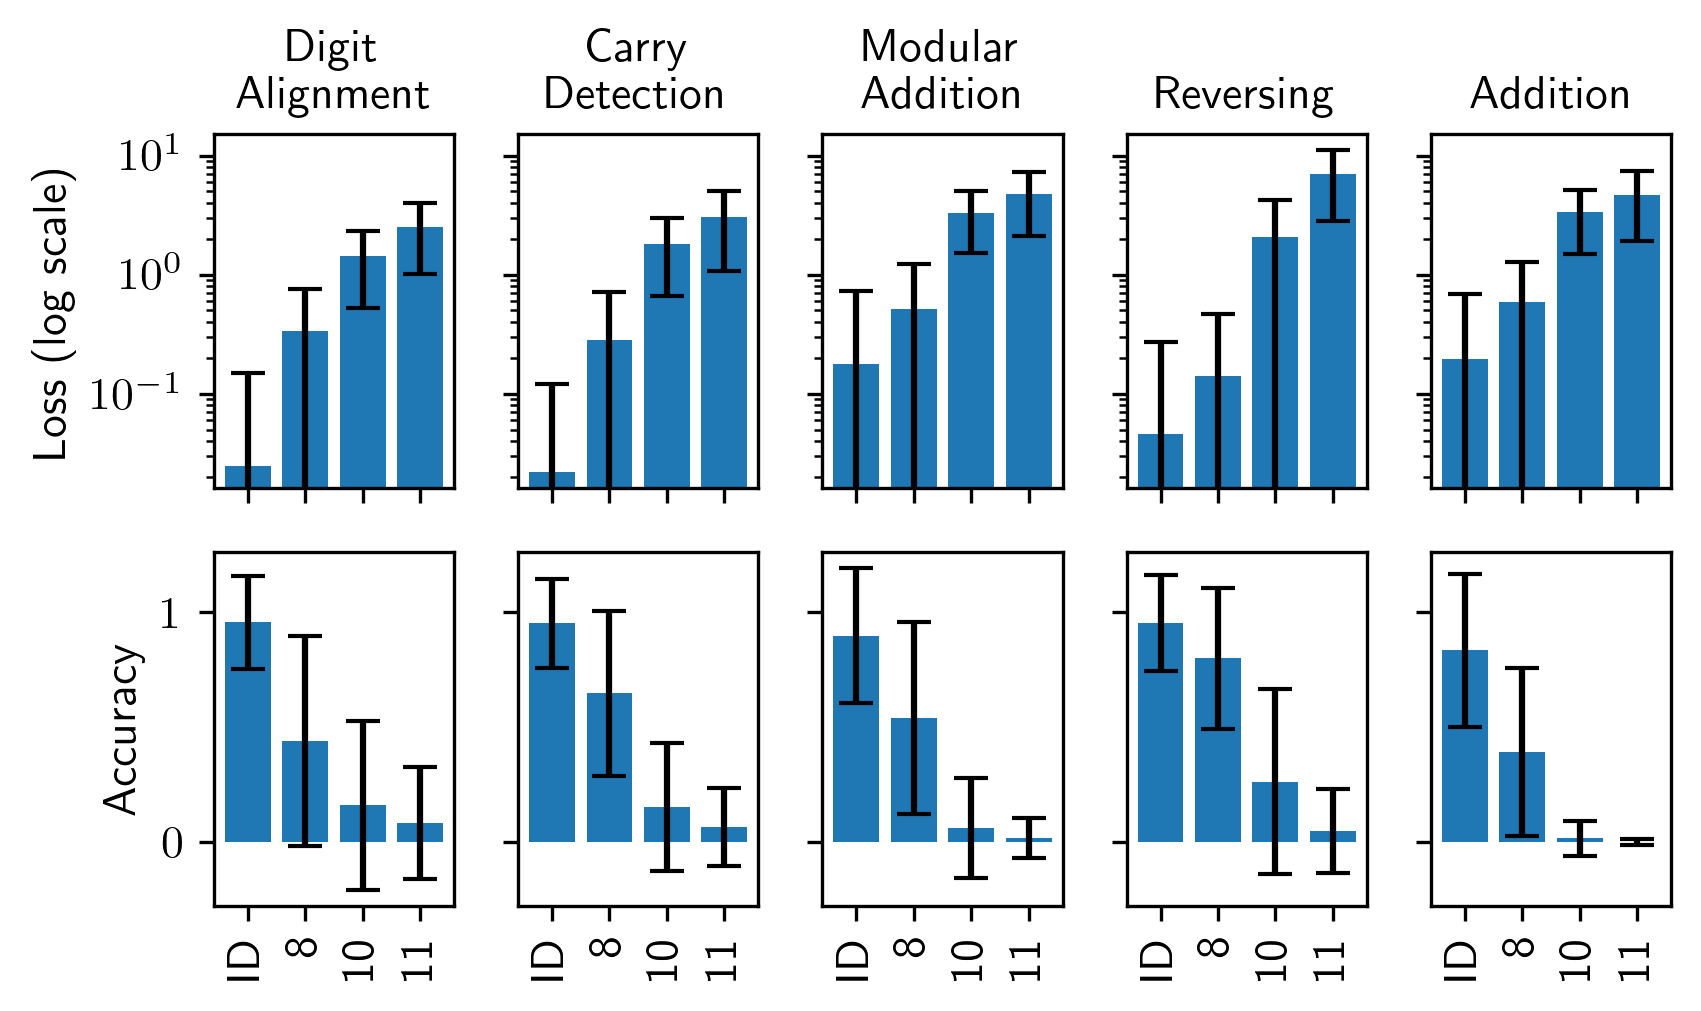
\includegraphics[width=0.7\linewidth]{fig/subtask_difficulty.png}
    \end{figure}
    \begin{itemize}
        \item Modular addition and digit alignment are the most challenging sub-tasks
        \item Significant variability in performance across different sub-tasks
    \end{itemize}
\end{frame}

\end{document}
